\chapter{Programming Languages}

\section{Programming Languages}
\begin{description}
    \item [Machine languages:] interpreted by the hardware itself
    \item [High-level languages:] interpreted by another program or compiled into another language
    \begin{itemize}
        \item Abstracts away system details
        \item Creates independence from hardware and operating system
    \end{itemize}
    \item [Syntax:] legal statements and expressions in the language
    \item [Semantics:] execution/evaluation rules for those statements and expressions
\end{description}

\section{Parsing}
\begin{itemize}
    \item Parsing: turning text into an expression
    \item Syntactic analysis: identifying the hierarchical structure of an expression
    \item Evaluation: the computation of the value of an expression
\end{itemize}

\section{Interpreters}
\begin{itemize}
    \item Programs specify the logic of a computational device
    \item An interpreter is a \emph{general computing machine}
\end{itemize}
\medskip
\begin{figure}[H]
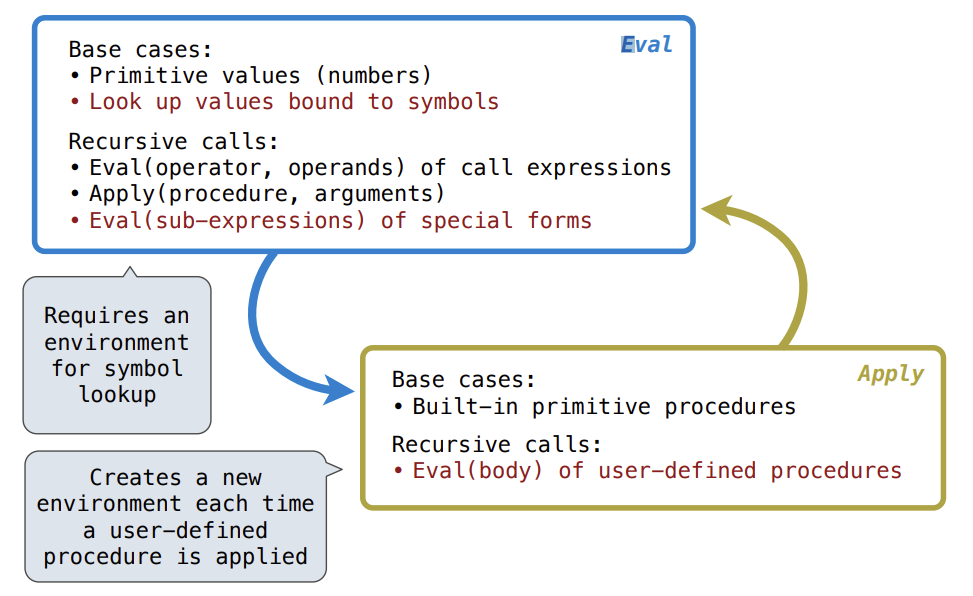
\includegraphics[width=0.8\linewidth]{figures/structure_of_an_interpreter.png}
\caption{Interpreter Structure}
\end{figure}